\section{iPad}
\label{sect:ipad}

The iPad 2 (hereafter simply ``iPad'') is a device about 7.3x9.5x0.3 inches with
a 1024x768 pixel touch screen \cite{ipad:specs}. The touch screen can detect
more than one human finger at a time, allowing for actions such as zooming to be
accomplished with natural gestures using two or more fingers.

The iPad runs iOS, a UNIX-based operating system which presents one fullscreen
application at a time and provides multithreading, persistent storage, wireless
network access, and other services.

This section describes iPad-specific user interface concepts that iPathCase
uses.

\subsection{Basics}
\label{sect:ipad_basics}

The iPad has a display resolution of 1024x768 pixels. Unlike traditional
computer displays, the iPad is designed to be held in any orientation, with the
display's contents rotating and resizing to fit the user's perspective. There
are four possible orientations, but the shortcuts ``landscape'' and ``portrait``
suffice for describing and implementing most interfaces \cite{ios:hig}.

\begin{table}[ht!]
    \centering
    \begin{tabular}{ | p{1in} | p{3in} | }
        \hline
        Gesture & Action
        \\ \hline
        Tap & To press or select a control or item (analogous to a single mouse click).
        \\ \hline
        Drag & To scroll or pan (that is, move side to side). To drag an element.
        \\ \hline
        Flick & To scroll or pan quickly.
        \\ \hline
        Swipe & With one finger, to reveal the Delete button in a table-view row or to reveal Notification Center (from the top edge of the screen).  With four fingers, to switch between apps on iPad.
        \\ \hline
        Double tap & To zoom in and center a block of content or an image.  To zoom out (if already zoomed in).
        \\ \hline
        Pinch & Pinch open to zoom in.  Pinch close to zoom out.
        \\ \hline
        Touch and hold & In editable or selectable text, to display a magnified view for cursor positioning.
        \\ \hline
        Shake & To initiate an undo or redo action.
        \\ \hline
    \end{tabular}
    \caption{\label{table:ipad_gestures}Common iPad gestures from ``The iOS Human Interface Guidelines''
    \cite{ios:hig}.}
\end{table}

The model for user interaction events in iOS is the \emph{gesture}. Table
\ref{table:ipad_gestures} lists some common gestures. Individual applications
are free to respond to these gestures however they see fit, but there is a basic
vocabulary of behavior that most applications follow.

\subsection{Views}
\label{sect:ipad_views}

The most basic component of an iPad interface is the \emph{view}. A view is a
rectangular region that is capable of displaying content, receiving events such
as gestures and device orientation changes, and delegating these tasks to
subviews. Views can contain buttons, toolbars, lists, other views, and arbitrary
graphical content. Nested views consist of a \emph{view hierarchy}.

A \emph{button} a view that renders itself in enabled, disabled, and pressed
states, and invokes some action when a touch is released inside its bounds.

\emph{Toolbars} are views that can be inserted at the top or bottom of another
view. They typically contain buttons, text labels, progress indicators, and
more.

A \emph{scroll view} contains another, larger view that the user can move
around with one or two fingers. For example, one might be used to display a
photo that is larger than the screen. Scroll views can be dragged around with
one finger, or zoomed out by pinching two fingers together. Tapping twice in the
same location typically zooms in on the tapped location.

One common use for the scroll view is in a \emph{table view}, used to display
lists of content. The user can scroll up and down the list and tap a row to
invoke some action.

\subsection{Container Views}
\label{sect:ipad_container_views}

Some types of views exist only to contain other views. One view of this type is
the \emph{popover}. A popover appears temporarily on the screen, allowing the
user to perform some quick interaction before dismissing it by tapping outside
its bounds.

\begin{figure}
    \center{
        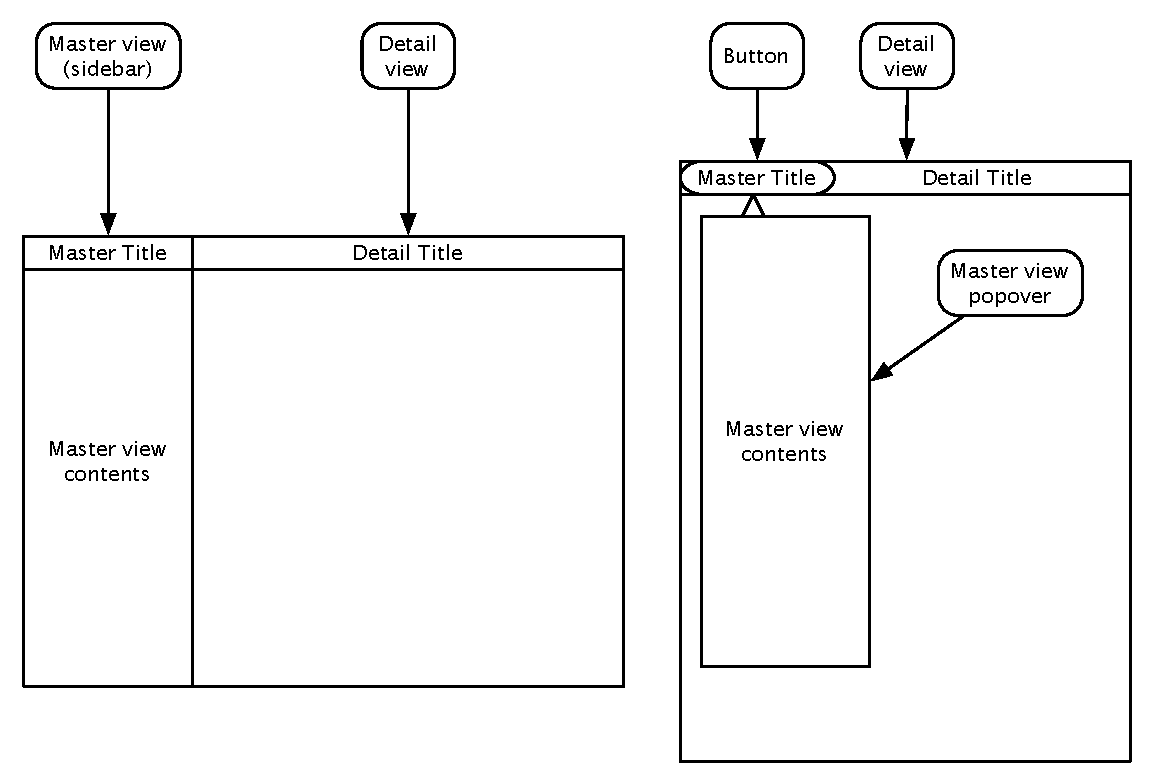
\includegraphics[width=\textwidth]{background/figures/master_detail}}
    \caption{\label{fig:master_detail} Master-detail interface in landscape
    and portrait orientations}
\end{figure}

The popover is a key component in the \emph{master-detail interface}, a common
arrangement of views in iPad applications. A diagram of the master-detail
interface is shown in figure \ref{fig:master_detail}. When the device is in a
landscape orientation, a thin view is shown to the left of a wide view. The thin
view, called the \emph{master view} or \emph{sidebar}, contains content for
navigating the application's data, such as a table view of email messages. The
wide view, called the \emph{detail view} or \emph{content view}, shows the
selection made in the master view.

When the device is in a landscape orientation, the detail view is resized to
fill the screen. A button on the left side of the top toolbar displays a popover
containing the master view.

\subsection{Navigation}
\label{sect:ipad_navigation}

Since iPad applications take the entire screen and can make only limited use of
multiple windows, the means of navigating between the screens of an interface
are very simple. The \emph{navigation stack} is a common metaphor. Like a web
browser, there is a ``back button'' in a toolbar at the top of the screen to
navigate to whatever screen was displayed before the current one.

The master view in a master-detail interface almost always uses one of these
navigation stacks. The view initially shows some top-level listing of the
application's data, such as mailboxes in an email account, with a toolbar at the
top containing a title for the view. Selecting one of these items pushes a new
view onto the stack, perhaps a list of message subjects, and a button appears
in the toolbar to go back to the mailbox list.
